\begin{figure}[tbp]
	\begin{center}
		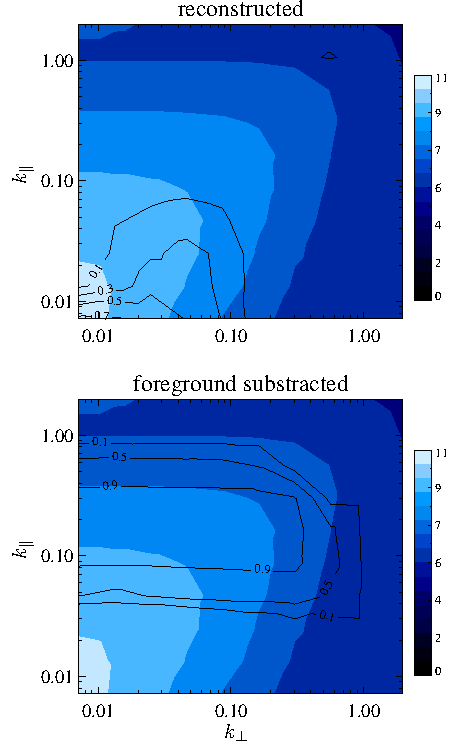
\includegraphics[width=0.48\textwidth]{vmode.pdf}
	\end{center}
	\vspace{-0.7cm}
	\caption{(Top) Contour shows the correlation $r(k_\perp,k_\parallel)$ between the real velocity field $v_z^{real}$ and $\hat v_z$ from the tidal reconstructed field; 
(Bottom) contour shows the correlation r between real velocity $v_z^{real}$ and $v_z^{fs}$ from the foreground substracted field. 
The background color indicating the level of powerspectrum of $v_z^{real}$ in logrithm, $lg(P_{v_z^{real}})$}. 
\label{fig:vmode}
\end{figure}

One of the main concerns about employing Cosmic Tidal Reconstruction is that it will import additional noise.
%In this section, we will demonstrate the distribution of old and new noises, and show
In this section, we will demonstrate that 
the newly recovered information on small $k_\parallel$ is far
more important than the loss of accuracy on larger k modes in this
problem, with typical foreground level, under current foreground substraction technology.

For comparison, we calculate the velocity field $v_{fs}$
directly from the foreground substracted field $\delta_{fs}$ following identical procedure.
In Fig.\ref{fig:vmode}, contours in upper panel show the 
correlation $r(k_\perp,k_\parallel)$ between the real velocity field
$v_z^{real}$ and foreground substracted velocity field $v_z^{fs}$; 
contours in lower panel show the
correlation r between $v_z^{real}$ and $\hat v_z$. 
The background color indicating the levels of velocity power spectrum
$P_{v_z^{real}}$. 

As we can see, although importing large noise to large k modes, 
the newly recovered small $k_z$ modes contain information that
corresponds to the highest level of $P_{v}$. 
These modes play a vital role in generating kSZ signals.

To better understand the behavior of kSZ signal, we write Eq.(\ref{eq:ksz}) in Fourier space.\begin{eqnarray}
\Theta(\bm{k_\perp})\equiv \Theta(k_x,k_y,0)=\int d^3k \delta(\bm{k}) v_z(\bm{k_\perp}-\bm{k})\,
\end{eqnarray}

Since $v(\bm{k})\propto \delta(\bm{k})\frac{k_z}{k^2}$, 
its amplitudes drops much faster than $\delta(\bm{k})$ when k gets larger, 
therefore could be consider as delta function. So $\Theta(\bm{k_\perp})\sim\delta(\bm{k_\perp})$

When the foreground contaminate the small $k_\parallel$ modes, as seen
from \ref{fig:vmode}, we lose the original peak in $v(k)$ and hence
select a totally different part of $\delta$ in mock kSZ signal.

From the blue dashed line in lower panel of Fig.\ref{fig:kSZ}, we can see the mock kSZ
signal calculated directly from a typical foreground substracted
fields($R_\parallel=15$ Mpc/h) will not
show any correlation with the real kSZ signal until $\ell$ gets greater
than $\sim300$.

On the other hand, aftering performing tidal reconstruction, we
recover the modes with small $k_z$ and tolerable $k_\perp$, 
which is close to the original peak in $v(k)$ and therefore enable us to get correlated signals.


However, we also have to noitice that by performing tidal reconstruction, 
we lost a portion of small $k_\parallel$ modes (reason discussed in \cite{2015:zhu}), 
which inhibits us from getting a better correlation.

If we consider a futuristic optimal case, when the foreground noise is
low and removed quite successfully.
Assume we have at least half density field structure remains at $k\sim
0.02$ Mpc/h, i.e. choose $R_\parallel=60$ Mpc/h.
Then we will be able to obtain a correlation of $\sim0.7$ at
$\ell\sim 300$ between the real kSZ sinal and mock kSZ signal directly
from the original field, this is certainly better than using tidal
reconstructed fields.

In all, the tidal reconstruction method is not designed to help us find the optimal correlation of the two signals, 
it is more like a safe belt that enable us to find a detectable correlation even when the measurement is not optimal. 
In the future, with telescope noises further supressed, 
better foreground substraction performed,
we should obtain more accurate correlation results between kSZ
signals and 21cm density field without any extra manipulations.
However, with current and upcoming facilities, the signal will
probably only be detected after tidal reconstruction.
The algorithm greatly advances the time for us to cross correlate
the two powerful probes---that is the value.


